% !TeX TXS-program:compile = txs:///latexmk/{}[-pdfxe -synctex=1 -interaction=nonstopmode -silent -outdir=Temp %.tex] 
%
\documentclass[bibstyle=super,font=empty]{Settings/XMUthesis}
%\documentclass[bibstyle=super,font=advance]{Settings/XMUthesis}
% !TeX root = ../XMU.tex

\author{林振炜}
\title{基于logistic模型和随机森林模型的财务造假因素的研究}
\date{\today} %二〇一九年二月二十八日
\class{2016级}
\studentnumber{15220162202239}
\department{经济学院}
\major{经济统计}
\advisor{冯峥晖 \quad 副教授}
%\otheradvisor{校外指导老师 \quad 副教授}
\team{经济学院~属性数据分析}
\fundteam{经济学院~属性数据分析}
\degree{本\quad 科}
\englishtitle{Research on Factors of Financial Falsification Based on Logistic Model and Random Forest Model}
\majorordouble{主修}
\lab{实验室}



\makeatletter
\let\xmutitle\@title
\let\xmuauthor\@author
\let\xmudate\@date
\makeatother
\usepackage{Settings/XMU-logo}
\usepackage{booktabs}
\usepackage[figuresright]{rotating}%这样才能保证奇数页偶数页都朝向右边
\usepackage{multirow}
\usepackage{dcolumn}
\usepackage{longtable}
\usepackage{amsmath}
\usepackage{graphicx}
\listfiles
\begin{document}

\frontmatter\xiaosi
\maketitle
%% !TeX root = ../XMU.tex
%%====================封面==========================

\begin{titlepage}
\begin{center}
\vskip \stretch{4}

\includegraphics[width=8cm]{xmu-flag}\\
\vskip \stretch{4}

   {\rmfamily  \bfseries \xiaoer 
   	 \the\degree  \quad 毕\quad 业\quad 论\quad 文\quad 
%   	 \quad 综\quad 述\quad 与\quad 翻\quad 译   
}\\ \vskip \stretch{2} 
   {\rmfamily \bfseries  \sanhao 
   (\the\majorordouble) \\
} \vskip \stretch{3}

   {\sffamily \bfseries \erhao 
		 \xmutitle 
}\vskip \stretch{3}

	{ \rmfamily \bfseries \sanhao
		 \the\englishtitle
}\vskip \stretch{2}
	
	\vskip \stretch{1}
	{ \sffamily  \sihao % \heiti 
		\begin{tabular}{rl} 
			姓\qquad 名: & \xmuauthor \\
			学\qquad 号: & \the\studentnumber \\
			学\qquad 院: & \the\department \\
			专\qquad 业: & \the\major \\
			年\qquad 级: & \the\class \\
			校内指导教师: & \the\advisor \\
			校外指导教师: & \the\otheradvisor\\
		\end{tabular}%
	}
	\vskip \stretch{2}
	\rmfamily\mdseries\sihao
	\vskip \stretch{5.5}
	\xmudate
	\vskip \stretch{2}
\end{center}
\end{titlepage}
\cleardoublepage
% !TeX root = ../XMU.tex
\chapter*{厦门大学本科学位论文诚信承诺书}
\setcounter{page}{1}
\begin{doublespace}

{\sihao
	
	本人呈交的学位论文是在导师指导下独立完成的研究成果。本人在论文写作中参考其他个人或集体已经发表的研究成果,均在文中以适当方式明确标明,并符合相关法律规范及《厦门大学本科毕业论文(设计)规范》。
	
	该学位论文为(\the\team%
	)课题(组)的研究成果,获得
	(%
	\the\fundteam)课题(组)经费或实验室的资助,
	在(%
	\the\lab)实验室完成。(请在以上括号内填写课题或课题组负责人或
	实验室名称,未有此项声明内容的,可以不作特别声明。)
	
	另外,本人承诺辅修专业毕业论文(设计)(如有)的内容与主修专业不存在相同与相近情况。
	
	\vspace{20pt}
	
	\hfill 学生声明(签名):\hspace*{4cm}\\
	\vspace{-10pt} 
	\hfill 年\hspace{26pt}月\hspace{26pt}日\hspace*{2cm}
}	
\end{doublespace}
%\clearpage
% !TeX root = ../XMU.tex

\chapter*{致谢} 

致谢语应以简短的文字对课题研究与论文撰写过程中曾直接给予帮助的人员(例如指导教师、答疑教师及其他人员)表示自己的谢意。
	
作为毕业论文提交时,应注意事项:致谢内容用小四号宋体。根据2016年2月施行的《厦门大学本科毕业论文(设计)规范》,致谢被放在论文起首。致谢结构一般分为三个部分:1,回顾;2,感谢; 3,承担责任以及献辞。第一部分可以简述论文写作的经历,所面对的挑战以及你如何应对。第二部分具体感谢在论文过程中给与你帮助的人。第三部分指出你将为自己的论文承担责任,如果你希望将此论文献给谁,可以在最后指出。致谢内容请亲自撰写,使其具备你个人的特色。抄袭任何模板内容是极其懒惰、没有意义、不负责任和错误的行为。
	

% !TeX root = ../XMU.tex
\chapter*{摘要}
%不要用我,我们,什么什么是当下的热点问题
%用本文,可以用被动语态
%科学的描述,引入要快,不用太长
%不要自问自答
%研究什么,用了什么方法研究,得出什么结论
%十句话左右

%presentation不要按论文的格式定
%建议直接抛出什么问题

由于我国证券市场发展时间相对较短,相关监管政策不健全等原因,上市公司财务造假仍呈现高发态势。为实现对财务欺诈行为进行准确预测,本文基于2018年上市公司的财务数据,构建了logistic模型和随机森林模型作为预测模型。logistic模型研究发现,中国的上市公司往往会选择通过对营业成本进行改动以对财务报表进行粉饰;在偿债能力越强的公司,其财务主管领取薪酬会更加减少财务造假的可能。随机森林模型的研究发现,利润总额增长率和可持续增长率是判别一个公司是否产生财务造假重要指标。

本文的研究为中国上市公司的财务造假识别提供了新的角度与方法,建立的模型有利于资源配置优化。为审计师审计财务造假提供了新的参考依据。	

\keywords{财务造假;logisitc模型;随机森林模型;营业成本;偿债能力;利润总额增长率;可持续增长率}	



\chapter*{\bfseries Abstract}

Due to the relatively short development time of China's securities market and the inadequacy of relevant regulatory policies, financial fraud in listed companies is still on the rise. In order to predict financial fraud accurately, this paper builds a logistic model and a RandomForest model based on the financial data of listed companies in 2018. 
The logistic model research found that Chinese listed companies often choose to decorate their financial statements by changing operating costs. In companies with stronger solvency, their financial officers will be more likely to receive financial remuneration when they receive compensation. The study of the Random orest model found that the total profit growth rate and sustainable growth rate are important indicators for judging whether a company has financial fraud.

The research in this paper provides a new perspective and method for the identification of financial fraud in Chinese listed companies. The model established is conducive to the optimization of resource allocation. It provides a new reference for auditors to audit financial fraud.

\englishkeywords{financial fraud; logisitc model; RandomForest model; operating cost; debt service ability; total profit growth rate; sustainable growth rate}


\xmutableofcontents
\mainmatter%
\pagestyle{fancy}
% !TeX root = ../XMU.tex
\chapter{引言}{Introduction}

%以下所述内容基本来自于 徐延的基于数据挖掘的财务。的研究,在查重前需要不断进行修改


中国的股票市场自1989年成立以来历经40年时间。在此期间,上市公司数量和总体规模 增长迅速,为我国经济发展注入了强劲动力。但是由于我国证券市场发展时间相对较短,相关监管政策不健全等原因,上市公司财务造假仍呈现高发态势,损害了投资者的切身利益, 影响了中国证券市场的健康稳定发展。因此,如何对上市公司财务造假问题进行精准识别和 有效预警就成为了监管层、机构投资者和个人投资者共同关注的问题。


财务造假一直是与财务报告相伴相生的一个问题,也是困扰监管层、金融业界和投资者多年的难题。某些企业出于粉饰公司业绩、提升投资者信心或逃避监管等目的,通过虚增交易、隐瞒相关信息、篡改财务数据等手段进行财务造假。常见手段包括特殊交易的不当核算(如对债权、债务重组以及关联交易的错误核算)、错用会计准则以及虚构交易、资产负债造假等等。这种行为不仅影响了投资者对公司情况的正确判断,还挑战了法律监管的权威。财务造假的“爆雷效应”还容易导致重大金融风险。因此,如何对上市公司财务造假问题进行精准识别和有效预警成为了各方面共同关注的问题。


回顾国外证券市场的发展史,我们可以发现,财务造假的先例可以追溯至英国南海公司的财务造假案,这起案件也被认为是非官方审计的开端。近几十年来,即使在监管体系较为完善的发达国家资本市场,上市公司财务造假案件也时有发生。其中,美国Enron公司\cite{noauthor_2002:_nodate}财务造假案影响较为巨大。


与发达国家相比,我国的证券业务开展时间较晚,部分上市公司抱有侥幸心理,各种违规现象时有发生。从违规类型来看,其中相当一部分属于财务造假。其中不仅有蓝田股份等典型案例,也有北大荒、雅百特等近年来新出现的案例。


对上市公司财务造假案例进行分析后,有研究者认为,只要公司的内部控制失效,公司管理层凌驾于内控体系之上,任何公司都有发生财务舞弊的可能,只是财务舞弊的手段和隐蔽性各有不同。


% 总的来看,从事高风险业务(农业、制造业、能源行业等)、拥有高风险财务结构的公司是财务舞弊现象的高发领域,被审计机构出具保留意见报告甚至不发表意见是财务造假的强烈信号。从造假动机来看,公司财务造假主要分为两种情况。在公司准备上市的阶段,出现财务造假主要体现在公司IPO的申请材料中,通过财务造假以满足《证券法》中关于公司上市的条件。公司上市后,出现财务造假的主要目的是美化公司业绩、提升投资者信心,以抬升股价,或为了避免退市等。因为公司上市前的数据获取存在较大难度,本文主要研究对象为公司己经成功上市后,处于上述目的而进行的财务造假行为。从造假手段来看,最常见的就是虚增交易。上市公司通过伪造单据、伪造合同虚构原本不存在的交易事项,以此形成虚假的收入和利润,这种方法可以快速改善公司财务报表中的收入和利润,形成公司发展态势较好的假象。另外,还有的公司通过虚增资产的方式进行财务造假,具体表现在对某些资产的估值严重偏离公允价值,以此达到虚增公司资产的目的。还有的公司通过提前确认收入的方式虚增收入,或者隐瞒重大事项等方式进行财务造假。特别是关联公司之间的交易问题是重灾区,控股公司和公司之间的关联交易常常偏离公允价格,以实现操纵上市公司利润的目的。从处罚力度来看,发达国家对上市公司财务造假的打击力度较大,不仅公司受到处罚,董事会成员和高管也会面临来自法院的刑事指控。另外,相关的会计师事务所和投行也会面临监管部门和司法部门的严厉处罚,总的来看违法的成本较高。在我国,相关法律法规对上市公司财务造假的处罚相比西方国家要偏轻,对相关责任人继续从业的限制规定时间也较短,导致一些公司仍然冒着违法风险进行财务造假。

本文尝试构建一个公司财务造假风险识别模型,为财务造假的识别提供技术支持和一定辅助。从资本市场及其参与者角度来看,本文的研究有以下几方面的现实意义。

首先,促进上市公司规范经营。加强对上市公司财务造假的识别,将提升上市公司的违法成本,可以促进上市公司和规范经营和真实披露,通过规范经营来获取经营业绩,而非通过财务造假来获得有吸引力的财务数据。

第二,提高资本市场效率。上市公司财务造假可能导致资本市场信息不真实,降低资本市场效率。因此加强对上市公司财务造假的识别有助于真实准确反映企业经营状况,提升资本市场效率,促进资本市场健康稳定发展。

第三,强化监管能力。以往的财务造假识别往往基于审计人员的主观判断,主要来自于审计人员对三张财务报表之间的逻辑关系进行推断分析,找出矛盾点和可疑点,从而对财务造假行为进行识别。但是这种识别方法也存在着一些不足,如耗时长、成本高、错误率和遗漏率高、过度依赖个人经验、缺乏统一标准等问题。因此,引入效率和准确率更高的算法和设计对于财务造假的精准识别具有重要意义。本文对上市公司财务造假识别的研究,将有助于监管部门加强对上市公司财务造假的预警和监测,提升违法成本,促使上市公司如实反映经营业绩。

第四,保护上市公司和投资者利益。在市场参与者层面,研究财务造假识别对维护上市公司和投资者利益都具有重要意义。财务数据是投资者进行投资决策的主要依据之一,篡改后的财务数据往往使得公司显得更有发展前景,对于证券投资者行为会产生误导,最终导致投资损失。对于上市公司而言,如果财务造假行为得不到有效遏制,就会在市场中引起“劣币驱逐良币”效应,损害上市公司利益。因此加强对上市公司财务造假识别的研究实质上有助于保护市场参与者的切身利益。
% !TeX root = ../XMU.tex
\chapter{文献综述}{Literature Review}

%需要讲出自己的论文有什么贡献,highlight your study's contribution
%一定要好好调研有没有人做过一样的
%ABC考虑了,但有一些问题没有透
%DEF考虑了,但是没有考虑透
%我考虑了,而且有意义
%不但要自己写文献综合,还要讲其优缺点
%用实证的角度来说明最新的造假手段

\section{财务造假原因综述}{Summary of Financial Fraud Reasons}

关于财务造假的成因,国外研究者提出了三角理论、GONE成因理论等。\citep{cresscy1973other}提出著名了财务造假三角理论,企业进行财务造假的诱因主要由三个方面,即压力、机会和自我接受。压力即代表了目前公司遇到问题的紧迫性,如利润不达标即将暂停上市、公司收入降低影响股价、公司现金流紧张等,在这种情况下,公司进行财务造假就有了行为上的动机。

%机会即公司内部管理制度的缺失,给财务造假行为提供了客观条件。自我接受(也称自我合理化)是指公司财务造假所使用的借口,如帮助公司暂时度过难关、维护股民利益等,这是公司管理层策划财务造假时的主管心态。这三个诱因一个是动机,一个是条件,一个是目的,少了任何一项,都无法支撑企业的财务造假行为。

\citep{bologna1993accountant}提出GONE\footnote{GONE由四个单词:greed,opportunity,need, exposure首字母组成}成因理论,也被称作“四因子理论”.该理论认为,公司财务造假的原因主要可以分为贪婪、机会、需要和暴露四个因子组成。此理论把个体的主观因素归为贪婪和需要,阐述了造假者的动机;机会和暴露更多是指财务造假的客观条件,即内控机制不完善带来的造假机会和造假行为被发现和惩罚的可能性。这几类因素从不同的层面影响公司的决策行为,最终造成了财务造假行为的产生。企业董事会或管理层有不良动机,有粉饰公司经营状况现实需要,且公司客观条件可以进行财务造假,且事后不易被发现,那么企业就可能对公司的经营情况进行虚假的说明。

在GONE理论提出后,后续的研究不断对其进行完善。如财务造假因子理论把GONE理论中的成因分为主观和客观,主观条件是指个人的道德品质、造假动机等,客观条件是指公司内控严格程度、被发现的可能性以及惩罚力度等。两类因素共同作用,决定了一个公司是否会进行财务造假。

在国外理论研究较为完善的基础上,近年来国内学者对上市公司财务造假也进行了研究。如\citep{Mei}以2006年至2015年因财务造假受到监管机构处罚的上市公司为样本进行研究,发现公司财务造假的成因可以是为了成功进行IPO或取得增发资格、对投资者隐瞒经营状况、防止出现ST、操纵股价等。


\section{财务造假识别研究综述}{Review of Research on Financial Fraud Identification}

财务造假的识别研究一直与财务造假本身的研究是相伴相生的,数十年来,国内外研究者己经对此问题进行了深入的研究和讨论,取得了一系列研究成果。相关研究主要分为三个阶段。

第一阶段是案例分析和特征总结,研究者主要对上市公司财务造假的典型案例进行分析比较,归纳总结这些公司及其财务数据多一些特征和矛盾点,研究变量和研究方法较为单一。\citep{pavlovic_fraud_2019}将Benford定律\footnote{由统计学家Benford于1938年提出,得出人们在处理的数据中,1-9作为首位数出现的概率是不同的}应用于财务造假的研究,利用塞尔维亚工商局2008年-2013年的数据,说明财务数据中,若第二个数字明显偏离Benford定律,那么有可能是公司对财务数据进行了改动。

第二阶段是建模分析,研究者开始由定性研究转为定量研究,通过建立数学模型对公司财务数据进行分析研判,从中寻找财务造假的痕迹。如\citep{md_nasir_real_2018}使用SCM(Securities Commissions of Malaysia)和Bursa Malaysia数据库对马来西亚上市公司的2001年到2008年的财务造假行为建立时间序列预测模型,进行实证分析。研究结果表明,在财务造假发生的前四年,盈余管理往往是非常有效的;生产成本在财务造假公司与非财务造假的公司的显著不同往往只发生在财务造假发生的前两年;Malaysia的上市公司往往喜欢通过操纵应计费用项目来进行财务造假等;\citep{gao_go_2017}通过实证研究表明财务造假的过程中往往伴随着外部董事的异常换手率,而且在此期间的换手率还同时与上市板块,会议频繁程度,以及财务高管的数量有关,研究还发现财务问题较多的公司其公司高管的离职率也会越高。在国内,\citep{liao_corporate_2019}实证研究表明,中国的企业社会责任可能是减少公司欺诈发生的有效途径。

第三阶段是大数据运用。随着信息技术的发展研究者开始使用数据挖掘技术对公司财务造假问题进行研究,取得了一定的研究成果。\citep{tseng_quadratic_2005}使用logistic模型研究财务报表风险甄别,得出logistic模型优于判别分析模型;\citep{chen_enhancement_2017}建立SVM模型检测财务造假,结果表明SVM模型的预测效果较好;\citep{abbasi_metafraud:_2012}使用在包含数千家合法和欺诈性公司的数据上进行了一系列实验,得出其使用的meta-learning(元学习)框架在对于财务欺诈具有较好的效果。结果表明,框架的每个组成部分均对其整体有效性做出了重要贡献,额外的实验证明了元学习框架相对于最新的欺诈检测方法的有效性。此外,该框架会生成与每个预测相关的置信度分数,这可以前所未有地促进财务欺诈检测性能,并可以作为有用的决策辅助工具。国内使用数据挖掘算法研究财务造假的研究发展仍较为缓慢,\citep{LU}应用logistic模型、判别分析模型、神经网络模型等对123家上市公司财务造假样本与非财务造假样本进行分类预测,得出logisitc模型的预测效果较好,\citep{MingLi}应用主成分分析方法和CART算法建立财务风险预测模型,\citep{mixedcore}通过线性组合构造混合核函数,建立基于混合核学习的支持向量机财务欺诈预测模型,与单核的支持向量机模型相比,其模型的鲁棒性与识别精度都有所提高。

\section{研究评述}{Research Review}
国外财务报表造假的甄别的研究方式相对于国内更加成熟,但是建模的样本数据具有特定的西方国家市场经济环境,并没有具体结合中国的国情,存在一定的局限性,模型指标的构建缺乏通用性,因此模型的应用推广能力不足,在解决我国实际问题中预测效果并不理想。

机器学习算法的预测能力非常强,但是在解释性角度有一定的不足。

鉴于此,本文在国内外研究的基础上,对财务报表数据进行统计分析,从财务盈利能力、运营能力、资产管理效率等角度,并引入一些用于判断财务造假的账目数据。本文的主要目的在于探究中国上市财务造假最容易发生在哪些账目,以及如何尽量提高准确率以达到更好的财务监管的目的。
% !TeX root = ../XMU.tex
\chapter{样本选取和变量选择}{Sample Selection and Variable Selection}

\section{数据来源}{Data Sources}
本文从2018年中国上市公司财务年报和相关违规信息数据中提取样本,数据主要来源于国泰安(CSMAR)数据库,所使用的财务造假公司信息主要从国泰安数据库的公司研究违规信息数据中提取,构建模型所用的自变量指标数据主要来自于国泰安数据库的公司研究系列,并使用Wind数据对其进行了补充。

\section{样本选取}{Sample Selection}
国泰安金融数据库对上市公司违规性质的分类共有16类,具体分类有
\begin{table}[!ht]
	\centering
	\begin{threeparttable}[b]
		\footnotesize
		\caption{国泰安金融数据库企业违规分类表}
	\begin{tabular}{cc|cc}
		\toprule
	违规编码  & 违规行为        & 违规编码  & 违规行为     \\ \bottomrule
	P2501 & 虚构利润        & P2509 & 擅自改变资金用途 \\
	P2502 & 虚列资产        & P2510 & 占用公司资产   \\
	P2503 & 虚假记载(误导性陈述) & P2511 & 内幕交易     \\
	P2504 & 推迟披露        & P2512 & 违规买卖股票   \\
	P2505 & 重大遗漏        & P2513 & 操纵股价     \\
	P2506 & 披露不实(其它)    & P2514 & 违规担保     \\
	P2507 & 欺诈上市        & P2515 & 一般会计处理不当 \\
	P2508 & 出资违规        & P2599 & 其他       \\ \bottomrule
	\end{tabular}
	\label{Fraud_type}
\end{threeparttable}
\end{table}

在表\ref{Fraud_type}中
%下面的内容是引用《基于数据的财务造假的研究》
本文直接把虚构利润和虚列资产的违规行为全部归为财务造假\cite{Research-on-Corporate-Financial-Fraud-Identific-ation-Model-Based-on-Data-Mining}。对于其他的几种违规行为,需要结合具体违规行为进行判断,最终得到了22个造假样本。

再结合各上市公司的年度审计报告中审计师给出的意见,包括标准无保留意见、保留意见、否定意见、无法发表意见、无保留意见加事项段、保留意见加事项段,本文对给出保留意见、否定意见、保留意见加事项段的事项进行审阅,最终认定有极强的造假嫌疑的样本共120个,无造假嫌疑的样本有3088个。

\section{变量选择}{Variable Selection}
\subsection{初步变量选择}{Preliminary Variable Selection}
本文参照GONE成因理论,再结合公司财务造假的手段等因素。从公司的财务数据、治理结构、造假动力与造假表现四个方面进行构建变量。

在财务数据的分类构建中,本文参照了国泰安数据库——公司研究的分类方法,从公司偿债能力、盈利能力、经营能力、发展能力4个方面构建财务数据指标,其中偿债能力选取了流动比率、速动比率、资产负债率、经营活动产生的的现金流量净额/负债和,经营能力选取了存货与收入比、流动资产与收入比、总资产周转率,盈利能力选取了营业毛利率,发展能力选取了资本保值增值率、利润总额增长率、可持续增长率。

在治理结构的分类构建中,本文股权集中度以及监管层的持股比例进行描述。

在造假动力的指标构建中,由于高层管理人员的报酬与财务业绩或公司股票的市场表现挂钩\cite{Research-on-the-Influencing-Factors-of-Jin-Chao's-2013-Financial-Statement-Fraud}本文选取了财务类高管是否在上市公司领取薪酬这个二值变量。

在造假表现方面,由于上市公司财务造假多围绕提升业绩展开,造假手段多样,主要有虚增收入、减少成本费用等\cite{Zhan-Hongyan-Common-Methods},故本文选取了管理费用增长率、营业总成本增长率、销售费用增长率、坏账准备计提比例的变化率、2018年坏账准备比例这5个变量,最终得到初始变量选取情况表 \ref{Initial}中

%这个表格太宽了,需要加入参数\footnotesize{}
% Please add the following required packages to your document preamble:
%、、引用要先写caption再写label

\begin{sidewaystable}[!ht]\footnotesize{}
	\centering
	\caption{初始变量选取情况表}
	\label{Initial}
	\begin{tabular}{ccc|c}
	\toprule
	指标类型                  & 指标代码 & 指标名称               & 指标计算方法                                                                              \\ \toprule
	\multirow{4}{*}{偿债能力} & liquidity\_ratio   & 流动比率               & 流动资产/流动负债                                                                           \\
						  & quick\_ratio						  & 速动比率               & (流动资产-存货)/流动负债                                                                      \\
						  & assets\_liabilities
						  & 资产负债率              & 总负债/总资产                                                                             \\
						  & cash\_liabilities
						  & 经营活动产生的现金流量净额/负债合计 & 经营活动产生的现金流量净额/总负债                                                                   \\ \cline{2-4} 
	\multirow{3}{*}{经营能力} & inventory\_income
	& 存货与收入比             & 存货/总收入                                                                              \\
						  & assets\_income\_ratio
						  & 流动资产与收入比           & 流动资产/总收入                                                                            \\
						  & asset\_turnover
						  & 总资产周转率             & 收入净额/平均资产总额                                                                         \\ \cline{2-4} 
	盈利能力                  & operating\_margin
	& 营业毛利率              & 营业毛利额/主营业务收入                                                                        \\ \cline{2-4} 
	\multirow{3}{*}{发展能力} & capital\_preservation
	& 资本保值增值率            & 期末所有者权益/期初所有者权益                                                                     \\
						  & profit\_growth
						  & 利润总额增长率            & (本期利润总额-上期利润总额)/上期利润总额                                                              \\
						  & sustain\_grow\_rate
						  & 可持续增长率             & 资产收益率*收益留存率/(1-净资产收益率*收益留存率)                                                        \\ \cline{2-4} 
	\multirow{2}{*}{治理结构} &TopTenHoldersRate
	& 股权集中度              & 前十名股东持股比例之和(\%)                                                                        \\
						  & reg\_shareholding
						  & 监管层持股比例            & 监管层持股数/总股数                                                                          \\ \cline{2-4} 
	动力指标                  & get\_paid
& 是否领取薪酬             & \begin{tabular}[c]{@{}c@{}}财务类高管是否在上市公司领取薪酬\\ 1=在上市公司领取薪酬,2=未在上市公司领取薪酬\end{tabular} \\ \cline{2-4} 
	\multirow{5}{*}{财务表现} & management\_rate
& 管理费用增长率            & \begin{tabular}[c]{@{}c@{}}(管理费用本年本期金额—\\  管理费用上年同期金额)/(管理费用上年同期金额)\end{tabular}    \\
						  & operating\_cost
						& 营业总成本增长率           & \begin{tabular}[c]{@{}c@{}}(营业总成本本年本期金额—\\  营业总成本上年同期金额)/(营业总成本上年同期金额)\end{tabular} \\
						  & sales\_expense\_rate
						& 销售费用增长率               & \begin{tabular}[c]{@{}c@{}}(销售费用本年本期金额—\\  销售费用上年同期金额)/(销售费用上年同期金额)\end{tabular}    \\
						  & bd\_ratio
						  & 2018年坏账准备比例        & 
						  \begin{tabular}[c]{@{}c@{}}(2018年坏账准备计提数/2018年应收账款数)\\-(2017年坏账准备计提数/2017年应收账款数)  
						  \end{tabular}                                                                     \\
						  & bad\_debt18
						& 坏账准备计提比例的变化率       & \begin{tabular}[c]{@{}c@{}}(2018年坏账准备比例-\\ 2017年坏账准备比例)/2017年坏账准备比例\end{tabular}    \\ \bottomrule
	\end{tabular}
	\end{sidewaystable}





\subsection{数据预处理与数据描述}{Data Preprocessing and Data Description}

由于本文选取的的变量皆为比率变量,故排除了上市公司的体量大小对结果的影响。对于bd\_ratio,该数据来自于Wind,其不仅报告了2018年的坏账比例,而且还报告了该坏账持续的时间,从财务知识可以知道,坏账持续时间越长则其收回的可能性越低,即成为坏账的可能性越高。因此本文对来自不同年份的坏账进行了加权处理,对于年份越久远的坏账给予更高的权重。


在处理缺失值方面,对于除get\_paid和bd\_ratio即财务类高管是否领取薪酬和坏账计提比例其他数据选择用2017年的数据对其进行补足,如果2017年的数据没有,则用该行业的平均水平来代替\footnote{依据证监会2012版行业分类标准};对于get\_paid,如果没有找到当前财务主管是否领取薪酬,则选取其有报告的最高的管理层是否领取薪酬来代替;对于bd\_ratio的缺失值,本文选择将其为0代替,即2018年的坏账比例相对2017年来说明没有发生变化。


观察如表\ref{descriptive_statistics}所示,发现流动比率、速动比率、存货与收入比、流动资产与收入比、资本保值增值率、利润总额增长率、管理费用增长率、营业总成本增长率、销售费用增长率的最大值比上四分位数都大出10倍左右,出于对数据真实性考虑以及希望排除某些数据录入错误造成的影响,对这些异常值进行处理,\citep{winsorization}的研究表明在财务比率的异常值处理方面,winsorize\footnote{是一种处理离群值的方法,在公司金融、财务管理等微观领域应用非常广泛,将超出变量特定百分位范围的数值替换为其特定百分位数值的方法}处理具有非常好的效果。因此,本文采用了winsorize方法,将上述变量超出95\%分位数的值用其95\%分位数进行替代。

% Table created by stargazer v.5.2.2 by Marek Hlavac, Harvard University. E-mail: hlavac at fas.harvard.edu
% Date and time: 周五, 12月 20, 2019 - 14:58:31
\begin{table}[!htbp] \centering 
    \caption{描述性统计} 
    \label{descriptive_statistics}
  \begin{tabular}{@{\extracolsep{5pt}}lccccccc} 
  \\[-1.8ex]\hline 
  \hline \\[-1.8ex] 
  Statistic & \multicolumn{1}{c}{N} & \multicolumn{1}{c}{Mean} & \multicolumn{1}{c}{St. Dev.} & \multicolumn{1}{c}{Min} & \multicolumn{1}{c}{Pctl(25)} & \multicolumn{1}{c}{Pctl(75)} & \multicolumn{1}{c}{Max} \\ 
  \hline \\[-1.8ex] 
  liquidity\_ratio & 3,208 & 2.370 & 2.673 & 0.123 & 1.180 & 2.580 & 54.507 \\ 
  quick\_ratio & 3,208 & 1.902 & 2.414 & 0.081 & 0.799 & 2.032 & 41.266 \\ 
  assets\_liabilities & 3,208 & 0.421 & 0.197 & 0.017 & 0.265 & 0.561 & 0.993 \\ 
  cash\_liabilities & 3,208 & 0.176 & 0.348 & $-$2.213 & 0.022 & 0.259 & 3.770 \\ 
  inventory\_income & 3,208 & 0.404 & 1.837 & 0.000 & 0.099 & 0.327 & 83.662 \\ 
  assets\_income\_ratio & 3,208 & 6.468 & 251.986 & 0.068 & 0.696 & 1.576 & 14,236.340 \\ 
  asset\_turnover & 3,208 & 0.648 & 0.531 & 0.0001 & 0.357 & 0.800 & 9.663 \\ 
  operating\_margin & 3,208 & 0.307 & 0.183 & $-$0.728 & 0.181 & 0.397 & 0.990 \\ 
  capital\_preservation & 3,208 & 1.155 & 1.682 & 0.022 & 1.010 & 1.124 & 69.264 \\ 
  profit\_growth & 3,208 & $-$0.399 & 10.785 & $-$213.431 & $-$0.358 & 0.331 & 371.127 \\ 
  sustain\_grow\_rate & 3,208 & 0.040 & 0.141 & $-$0.977 & 0.018 & 0.089 & 1.592 \\ 
  TopTenHoldersRate & 3,208 & 60.209 & 14.726 & 10.890 & 51.227 & 69.755 & 100.970 \\ 
  bad\_debt18 & 3,208 & 53.899 & 12.819 & 0 & 50 & 61.5 & 91 \\ 
  bd\_ratio & 3,208 & 0.012 & 0.256 & $-$1 & 0 & 0 & 12 \\ 
  management\_rate & 3,208 & 0.298 & 2.346 & $-$0.737 & 0.049 & 0.309 & 125.092 \\ 
  sales\_expense\_rate & 3,208 & 1.723 & 73.196 & $-$1.000 & $-$0.001 & 0.315 & 4,133.569 \\ 
  Ownership & 3,208 & 1.860 & 0.809 & 1 & 1 & 2 & 8 \\ 
  operating\_cost & 3,208 & 0.418 & 8.991 & $-$0.829 & 0.038 & 0.299 & 504.738 \\ 
  reg\_shareholding & 3,208 & 0.115 & 0.178 & 0.000 & 0.000 & 0.196 & 0.823 \\ 
  \hline \\[-1.8ex] 
  \end{tabular} 
  \end{table} 


\subsection{多重共线性分析}{Multicollinearity Analysis}
由于财务报表数据本身所具有的内部逻辑性,本文初选出的指标之间也必然存在着某种程度的自相关性,这对模型估计的参数准确性会产生影响。因此,在代入模型之前,我们首先要分析多重共线性,把部分自相关性较高的变量剔除。

首先对所有变量进行VIF检验\footnote{VIF(方差扩大(膨胀)因子法)是通过考察给定的解释变量被方程中其他所有解释变量所解释的程度,以此来判断是否存在多重共线性的一种方法。}最终得到如表\ref{vif}所示,其中流动比率,速动比率、资本保值增值率、可持续增长率的VIF值大于10,可以认为其具有较强的多重共线性,最终去掉了流动比率与资本保值增值率这两个变量,得到的最终变量都通过了vif检验。而且根据两两之间的线性关系图如\ref{corrplot}所示(详见附录),两两之间的关系也是比较弱的。至此,我们的初步变量选择完成。


% Please add the following required packages to your document preamble:
% \usepackage{booktabs}
\begin{table}[]
	\centering
	\caption{VIF检验}
	\label{vif}
	\begin{tabular}{@{}c|l@{}}
	\toprule
	变量                 & VIF     \\ \toprule
	流动比率               & 83.047 \\
	速动比率               & 81.285 \\
	资产负债率              & 1.825  \\
	经营活动产生的现金流量净额/负债合计 & 1.454  \\
	存货与收入比             & 1.315  \\
	流动资产与收入比           & 1.014  \\
	总资产周转率             & 1.131  \\
	营业毛利率              & 1.330  \\
	资本保值增值率            & 10.679  \\
	利润总额增长率            & 1.407  \\
	可持续增长率             & 12.630 \\
	股权集中度              & 1.456  \\
	监管层持股比例            & 1.1279  \\
	是否领取薪酬             & 1.0539  \\
	管理费用增长率            & 1.130  \\
	营业总成本增长率           & 1.677  \\
	销售费用增长率               & 1.041  \\
	坏账准备计提比例的变化率       & 1.038  \\
	2018年坏账准备比例        & 1.083  \\ \bottomrule
	\end{tabular}
	\end{table}
%要讲清楚数据的来源与数据清洗的过程
%descriptive analysis要做,要和下一步有关系
% !TeX root = ../XMU.tex
\chapter{实证分析}{Analysis of Model Empirical Results}

%加上一个Z就不显著,说明Z可能与X强相关

% 通过对上市公司不同板块的分类,我们可以得到如\cref{board_fraud}所示
% \begin{figure}[!ht]
%     \centering
%     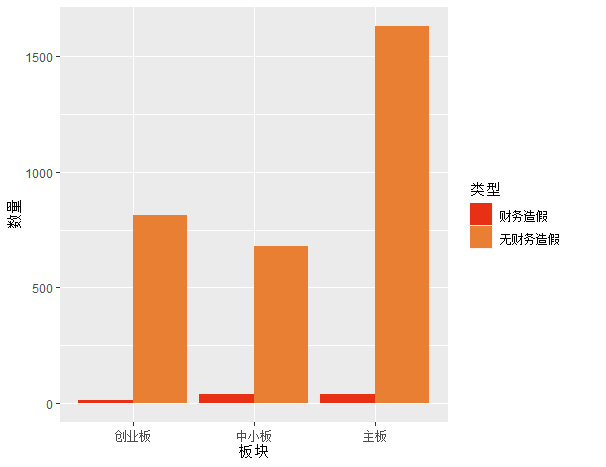
\includegraphics[scale=1]{Board_fraud}
%     \caption{不同板块的财务造假统计} \label{board_fraud}
%     \end{figure}
% 可以看到在不同的板块,财务造假的公司分类的还是比较均匀的,没有在某个板块财务造假的现象极为突出的情况存在

\section{数据平衡与样本重建}{Data Balance and Sample Reconstruction}
初步我们得到有极强的造假嫌疑的样本共120个,无造假嫌疑的样本有3088个,二者比例为1:25左右,存在较为严重的样本不平衡问题。对于这个问题的解决主要通过欠采样和过采样的方法,考虑到欠采样将导致样本的数据急剧下降,因此本文采用的过采样的方法进行解决。

本文采用SMOTE方法\cite{Chawla2011SMOTE}进行数据过采样,最终得到造假样本440条,非造假样本528条,二者比例接近1:1。

\section{Logistic模型实证分析}{Logistic Model Empirical Analysis}
\subsection{Logistic模型}{Logistic Model}
Logistic 回归模型是传统经典的分类方法,在因变量取值为二分类时进行回归分析,基本思路是通过 Logistic 非线性变换,利用极大似然估计的方法,通过Newton-Raphson方法进行迭代求解,求出系数的估计值,建立一个概率拟合函数。它是一个参数线性的判别类,用于解释一个二元变量与一个或多个度量自变量之间的关系 
\cite{agresti_introduction_2007}。


本文通过 Logistic 回归模型将自变量的取值代入到概率拟合函数,在二元值中通过预测因变量的概率取值,假设预测概率大于 0.5,则财务舞弊预测发生,预测概率小于 0.5,则财务造假预测不发生。概率取值为度量尺度,从而判断样本的所属类别进行二分类。

\subsection{Logistic模型的构建与实证分析}{Logistic Model Construction and Empirical Analysis}

%作这些回归的目的,探究中国上市公司的主要造假手段,以及在财务类高管领取与不领取报酬的公司,相同的造假手段是否存在异质性
%之前会报错的原因是下划线忘记用斜杠转义了

首先本文先对前文提到的变量共17个\footnote{排除了两个共线性变量liquidity\_ratio与capital\_preservation。},
进行建模得到一个完整的全模型,而后,根据AIC原则,采用向前和向后两种变量选择方法得到了相同的结果,再删除掉不显著的无关变量,最终得到了如表\ref{logistic_regression}中的方程(1),该方程的变量选择涉及到了我们所构建指标的各个方面,其中财务表现,发展能力,治理结构,动力指标,偿债能力这几个方面都有变量入选。

表\ref{logistic_regression}汇报了基于先前初步选择变量的结果。从方程(1)可以看出,在财务造假的表现方面,operationg\_cost显著为负的,即营业总成本增长,对于财务造假的预测具有明显的负效应。换句话说,中国的上市公司在财务造假的过程中,往往会选择通过即营业总成本减少以达到虚增利润的效果,而较少会通过计提坏账准备,减少销售费用和减少管理费用的方式;在发展能力方面sustain\_grow\_rate是显著为负的,而且其对最终财务造假的预测影响较大,说明一个发展前景较好的公司具有较低的财务造假的可能,这与之前的理论分析相契合;

% 在公司的治理结构方面,TopTenHolderRate的系数是显著为负的,说明从整个市场的来看,前十大股东的持股比例越高,其财务造假的风险反而越低,这与我们先前的理论似乎相违背,但是该指标的系数大小仅为

在方程(1)中财务类高管是否领取薪酬对于财务造假的预测是没有显著影响的,然而作为动力指标,不领取薪酬可能会导致更强的财务嫌疑,因为其报酬极有可能与公司的财务表现相挂钩,其主观动力会更强。

为探究在不同的财务指标下,财务类高管领取与不领取薪酬对财务造假是否存在不同影响,得到了回归方程(2)加入了get\_paid与quick\_ratio的交叉项,可以知道,财务类高管领取薪酬确实对财务造假预测有一定的影响,且其参数显著为负,表明财务类高管没有在上市公司领取薪酬,将会使降低财务报表造假预测的概率,即认为财务类高管没有领取薪酬的上市公司财务造假的可能会小于那些财务类高管领取薪酬的上市公司,并且该影响将会随着quick\_ratio的上升而弱化,当$quick\_ratio>1.318$,该影响将会由负转正。
% 对比方程(2)与方程(3)可以发现财务类高管领取薪酬对是否财务造假存在simpson悖论,即从整个中国上市公司整体环境来看,财务类高管领取薪酬对财务造假影响不显著,但是在不同的速动比率的公司,财务类高管是否领取薪酬对上市公司是否财务造假具有显著的影响,甚至随着速动比率的不断上升,其影响会由负转正。
速动比率衡量的是短期偿债能力,从衡量长期偿债能力的assets\_liabilities即资产负债率来看,结论也是类似的。速动比率是一个正向指标\footnote{正向指标指认为指标值越大,偿债能力越强,负向指标与之相反},资产负债率是一个负向指标。因此,同样对比方程(1)与方程(3)可以发现在不同资产负债率的公司,财务类高管是否领取薪酬对上市公司是否财务造假具有显著的影响,甚至随着资产负债率的不断上升,其影响会由正转负。因此这就说明了观点:在不同偿债能力的公司,财务类高管是否领取薪酬对上市公司是否财务造假具有显著的影响是不同的,偿债能力越强的公司,其财务类高管领取薪酬对财务造假的预测具有更强的负向影响,即认为财务类高管领取薪酬会减少财务造假的可能,而且这种影响在偿债能力强的公司将会更加显著。








%这个公式mathtype那边剪切格式要改一下,太长了


%R语言实证结果,需要将tabular改为longtable,并把前面的一些table内容删掉,并且要注意,tabular的东西只能放在一个页面当中
% 然后标题和label要用\caption{\label{tab:test}我的跨页表格}的格式写
% 通过\renewcommand\arraystretch{0.5}来调整行距,0.5就挺好的

\renewcommand\arraystretch{0.5}
  \begin{longtable}{@{\extracolsep{5pt}}lD{.}{.}{-3} D{.}{.}{-3} D{.}{.}{-3} } 
    \caption{\label{logistic_regression}回归结果}
    \\[-1.8ex]\hline 
    \hline \\[-1.8ex] 
     & \multicolumn{3}{c}{\textit{Dependent variable:}} \\ 
    \cline{2-4} 
    \\[-1.8ex] & \multicolumn{3}{c}{ViolationTypeID} \\ 
    \\[-1.8ex] & \multicolumn{1}{c}{(1)} & \multicolumn{1}{c}{(2)} & \multicolumn{1}{c}{(3)}\\ 
    \hline \\[-1.8ex] 
     get\_paid2 & 0.484 & -1.566^{**} & 2.863^{**} \\ 
      & (0.407) & (0.774) & (1.250) \\ 
      & & & \\ 
     quick\_ratio & 0.177^{***} & 0.160^{***} & 0.176^{***} \\ 
      & (0.061) & (0.059) & (0.060) \\ 
      & & & \\ 
     assets\_liabilities & 1.421^{**} & 1.525^{**} & 1.571^{**} \\ 
      & (0.632) & (0.630) & (0.637) \\ 
      & & & \\ 
     cash\_liabilities & -2.343^{***} & -2.371^{***} & -2.400^{***} \\ 
      & (0.475) & (0.480) & (0.479) \\ 
      & & & \\ 
     sustain\_grow\_rate & -7.302^{***} & -7.329^{***} & -7.321^{***} \\ 
      & (0.709) & (0.712) & (0.711) \\ 
      & & & \\ 
     TopTenHoldersRate & -0.012^{**} & -0.011^{*} & -0.011^{*} \\ 
      & (0.006) & (0.006) & (0.006) \\ 
      & & & \\ 
     operating\_cost & -0.361^{*} & -0.333^{*} & -0.319^{*} \\ 
      & (0.208) & (0.188) & (0.187) \\ 
      & & & \\ 
     get\_paid2:quick\_ratio &  & 1.188^{***} &  \\ 
      &  & (0.438) &  \\ 
      & & & \\ 
     get\_paid2:assets\_liabilities &  &  & -5.151^{**} \\ 
      &  &  & (2.517) \\ 
      & & & \\ 
     Constant & -0.249 & -0.309 & -0.353 \\ 
      & (0.512) & (0.510) & (0.514) \\ 
      & & & \\ 
    \hline \\[-1.8ex] 
    Observations & \multicolumn{1}{c}{968} & \multicolumn{1}{c}{968} & \multicolumn{1}{c}{968} \\ 
    Hosmer-Lemeshow X2 & \multicolumn{1}{c}{$47.229^{***}$} & \multicolumn{1}{c}{$48.862^{***}$} & \multicolumn{1}{c}{$47.947^{***}$} \\ 
    \hline 
    \hline \\[-1.8ex] 
    \textit{Note:}  & \multicolumn{3}{r}{$^{*}$p$<$0.1; $^{**}$p$<$0.05; $^{***}$p$<$0.01} \\  
  \end{longtable} 




\subsection{Logistic模型评价}{Logistic Model Evaluation}
本文通过变量选择得到了模型\cref{eq:last}其方程为:
  
% \[\begin{array}{ccccc}
%     \log it(\hat \pi ) =&- 0.0651 + 0.1544quick\_ratio + 1.2126assets\_liabilities\\
%     &  - 2.0919cash\_liabilities - 0.2404asset\_turnover\\
%      &  - 6.2771sustain\_grow\_rate - 0.00136TopTenHoldersRate\\
%      &+1.3843get\_paid + 0.2187management\_rate
%     \end{array}\]

\begin{equation}
    \begin{aligned}
        \log it(\hat \pi ) =&- 0.309 + 1.566get\_paid+0.160quick\_ratio + 1.525assets\_liabilities\\
    &- 2.371cash\_liabilities- 7.329sustain\_grow\_rate - 0.011TopTenHoldersRate\\
        &-0.333operating\_cost+1.188get\_paid2\times quick\_ratio
    \end{aligned} 
    \label{eq:last}   
\end{equation}

其中:$\log it(\hat \pi ) = ln(\frac{{\hat \pi }}{{1 - \hat \pi }})$

对上述模型,本文选择了常用的auc指标与混淆矩阵\footnote{其中$\pi_{0}$为样本比例0.545}对其预测能力进行评判。根据模型可得到如\cref{ROC}所示的ROC曲线图,其AUC值达到了0.8834,具有较好的识别财务造假的能力。为使得到的结果更加具有稳健性,本文接着采用了十折交叉检验\footnote{即将所有的数据随机切割成十份,依次选择其中九份作为训练集,剩下一份样本为测试集}的方式对样本进行切割为训练集和测试集,用训练集拟合模型参数,并用训练集进行检验预测能力,并将得到的混淆矩阵十次的结果取平均,得到如\cref{Confusion matrix}所示,其specificity的均值为0.911,sensitivity的均值为0.702,十次得到的auc取均值为0.886。综上,是可以认为我们建立得到的模型是具有较强的预测能力的。

\begin{figure}[!ht]
    \centering
    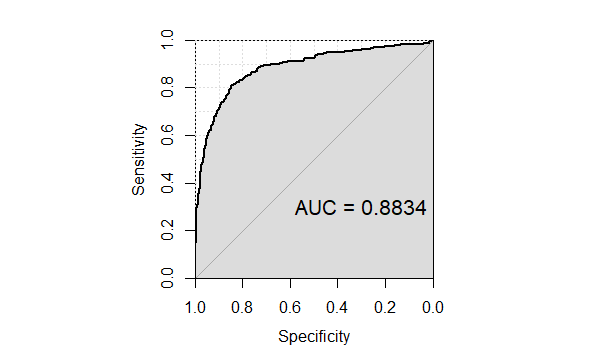
\includegraphics[scale=1]{ROC}
    \caption{logistic ROC} \label{ROC}
    \end{figure}

    % Please add the following required packages to your document preamble:
% \usepackage{multirow}
\begin{table}[!ht]
    \centering
    \caption{Confusion matrix}
    \label{Confusion matrix}
    \begin{tabular}{ccc}
        \toprule
    \multirow{2}{*}{Fraud In Reality} & \multicolumn{2}{c}{Fraud In Prediction} \\ \cline{2-3} 
                                      & T                  & F                  \\ \toprule
    T                                 & 40.0               & 3.9                \\
    F                                 & 15.5               & 36.6               \\ \bottomrule
    \end{tabular}
    \end{table}


\section{随机森林模型分析}{Random Forest Model Analysis}

为探究本文选择的变量在使用其他预测模型时仍然有较好的效果,本文选择了树模型对本文选择的变量进行预测,%下面这句是抄的
树模型包括决策树,随机森林,提升树等,其中随机森林(Randomforest),提升树作为一种组合分类器算法,在大样本、高维度特征和异常值数据上仍然能够保持较好的预测准确率,最终通过准确率的比较,本文选择了随机森林模型作为最终模型,在这项预测中,随机森林模型在多种树模型中具有明显的优点。

\subsection{随机森林模型}{Random Forest Model}
随机森林模型通过对树作相关处理,实现对袋装法树的改进。在随机森林中需对自助抽样训练集建立一系列决策树,但是在建立决策树时,每考虑树上的一个分裂点,都要从全部的p个预测变量中选出一个包含m个预测变量的随机样本作为候选变量。随机森林算法可以用于连续变量的预测,也可以用于分类型变量的预测,对于本文的二值变量的预测同样具有较好的效果\cite{james_introduction_2013}。
随机森林模型的决策树分类器的构建过程如下:
%抄的

(1)对原始数据集有放回的随机抽样,引导生成与原始实例集相同数量的样本,组成一定规模的随机子集,随机子集的规模对应随机森林的规模;

(2)在每个随机子集的生成过程中,可以证明,约有37\%的样本不会被采用,称为OOB(out of bagging)。并且,利用OOB进评估模型的训练损失,是一种无偏估计\cite{Breiman2001Random}。


(3)随机子集对应决策数根节点。在每个节点随机抽样样本特征,最后到达限制层数或者当每个叶节点是纯数据的时候,停止分裂。

\subsection{随机森林模型的选择与构建}{Selection and Construction of Random Forest Model}
本文采用前文提到的十折交叉验证来对进行模型的选择,通过对树的棵树进行调参,并采用十折交叉验证来计算其平均的准确度,最终得到三种模型的准确率的对比如图\ref{three_model}。从图中可以到随机森林算法的误差率是显著小于Bagging和Adaboost的,故最终选择了随机森林算法,找到其中使误差最小的树的棵数为505。
\begin{figure}[!ht]
    \centering
    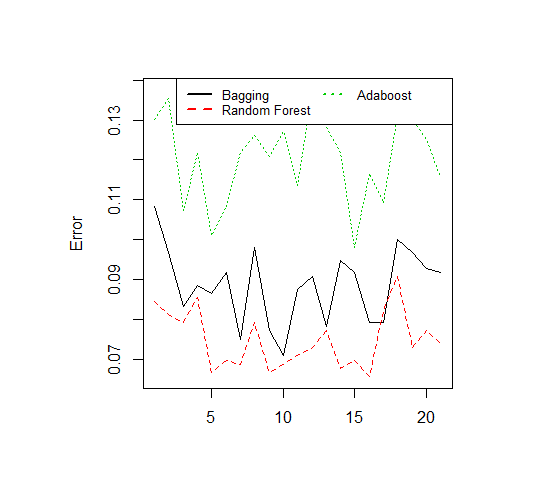
\includegraphics[scale=1]{three_model}
    \caption{模型平均误差图} \label{three_model}
    \end{figure}


\subsection{随机森林模型的评价}{Random Forest Model Evaluation}

使用准确率最高的参数即$ntree = 505$,$mtry = 4$建立随机森林模型可以得到其准确率达93.4\%。

对于上述模型,本文同样选择了常用的auc指标与混淆矩阵对其预测能力进行评判。根据模型可以得到如图\ref{randomforest_ROC}所示的ROC曲线,其AUC值达到了0.976,相对于logistic模型来说是显著的提升。同样使用十折交叉检验的方式对样本进行切割,并得到十次的平均混淆矩阵,得到如表\cref{confusion_}所示,其specificity的均值为0.900,sensitivity的均值为0.914,相对于logistic模型来说,其specificity的值没有明显的下降,但是sensitivity却有明显的提高。


\begin{figure}[!ht]
    \centering
    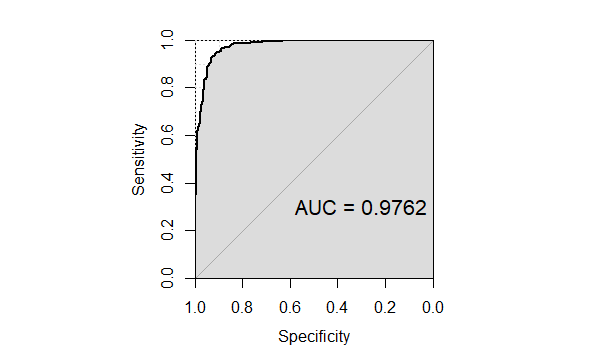
\includegraphics[scale=1]{randomforest_ROC}
    \caption{RandomForest ROC} \label{randomforest_ROC}
    \end{figure}

    % Please add the following required packages to your document preamble:
% \usepackage{multirow}
\begin{table}[!ht]
    \centering
    \caption{Confusion matrix}
    \label{confusion_}
    \begin{tabular}{ccc}
    \hline
    \multirow{2}{*}{Fraud In Reality} & \multicolumn{2}{c}{Fraud In Prediction} \\ \cline{2-3} 
                                      & T                  & F                  \\ \hline
    T                                 & 38.0               & 4.2                \\
    F                                 & 4.6                & 49.2               \\ \hline
    \end{tabular}
    \end{table}


对于随机森林模型为什么可以显著提高sensitivity的原因除了该模型可以解决非线性分类等模型本身的优势之外,其预测变量的选择与logistic模型选择的变量不同也是重要的一方面,如图\ref{importance}所示,可以看到在随机森林模型判别标准中利润总额增长率和可持续增长率是判别模型中最重要的变量,其中利润总额增长率在logistic模型甚至没有出现在最终选择的模型中。


\begin{figure}[!ht]
    \centering
    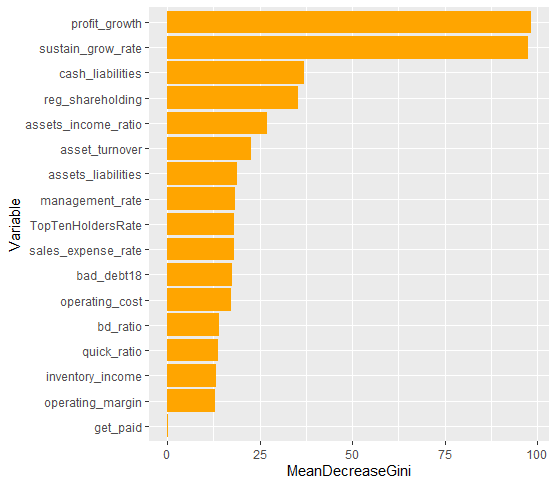
\includegraphics[scale=1]{importance}
    \caption{变量重要性排序} \label{importance}
    \end{figure}
% !TeX root = ../XMU.tex
\chapter{结论与局限性}{Conclusion and Limitation}
%就说方法本身有什么缺点
%基于模型的机制的调整
%进一步做可以做什么

% \section{算法}{Algorithm}

% 这是算法的插入示例,可能软件学院、信息科学学院这类的同学用得上吧。
% \begin{algorithm}
% 	\caption{My algorithm}\label{euclid}
% 	\begin{algorithmic}[1]
% 		\Procedure{MyProcedure}{}
% 		\State $\textit{stringlen} \gets \text{length of }\textit{string}$
% 		\State $i \gets \textit{patlen}$
% 		\BState \emph{top}:
% 		\If {$i > \textit{stringlen}$} \Return false
% 		\EndIf
% 		\State $j \gets \textit{patlen}$
% 		\BState \emph{loop}:
% 		\If {$\textit{string}(i) = \textit{path}(j)$}
% 		\State $j \gets j-1$.
% 		\State $i \gets i-1$.
% 		\State \textbf{goto} \emph{loop}.
% 		\State \textbf{close};
% 		\EndIf
% 		\State $i \gets i+\max(\textit{delta}_1(\textit{string}(i)),\textit{delta}_2(j))$.
% 		\State \textbf{goto} \emph{top}.
% 		\EndProcedure
% 	\end{algorithmic}
% \end{algorithm}

本文以2018年上市公司财务报表结合违规内容以及会计师审计意见的数据,考察了当前财务造假的财务表现,建造一个财务造假的预测模型。

\section{结论}{Conclusions}

logistic模型研究结果显示:中国的上市公司往往会选择通过营业成本进行改动来达到自己美化财务报表的目的;发展前景较好的公司往往具有较低的财务造假的可能;在偿债能力越强的公司,其财务主管领取薪酬会更加减少财务造假的可能。从对logistic模型的评价中我们可以发现,logistic模型对财务造假的预测效果总体来说并不是非常的好,尤其是甄别造假公司的确造假的准确率(sensitivity)并不是特别高。鉴于此,logistic模型对于统计解释有着较大的意义,但是对财务造假模型的预测仍然需要进一步的改进。

随机森林模型研究结果显示:机器学习算法对于财务造假的分类问题十分有效。其不论是在specificity和sensitivity两方面都表现的非常好。且该模型对于变量的选择也与logistic模型具有十分大的区别,认为利润总额增长率和可持续增长率是判别一个公司是否产生财务造假的最重要的两个指标。

\section{局限性}{Limitation}
会计账目中存在一些如人力资本、知识产权及专利技术等无形资产难以用货币衡量。会计报表遵循谨慎性原则,并没有包括未来企业价值和报表外的信息,如企业的社会责任的衡量。这些问题可能会影响控制变量的计算结果,进而影响模型分类的准确率与解释性。








































% \section{参看文献与引用}{Reference and citation}

% 一下是一些参考文献的引用。应该能有合适的。不合适可以修改。


% \cite{liuhaiyang2013latex,CTEX}

% \cite{XMU}

% \citet{liuhaiyang2013latex}

% \citep{liuhaiyang2013latex}
% %用这个引用格式,英文只能出现姓和年如:Borgja(2003),中文的就是全名
% %两个人
% %是这篇论文干了什么事,而不是这人干了什么事
% %研究这个问题的还有很多,见

% \citealt{liuhaiyang2013latex}

% \citeauthor{liuhaiyang2013latex}

% \citeyearpar{liuhaiyang2013latex}

\backmatter
\nocite{*}


%\bibliographystyle{IEEEtran}
% \clearpage
\phantomsection
\addcontentsline{toc}{chapter}{参考文献}
%总算找到怎么加英文的了是tce
\addcontentsline{tce}{chapter}{\rmfamily\bfseries Reference}


% \newcommand\Echapter[1]{
% 	\markboth{#1}
% 	\addcontentsline{tce}{chapter}{Reference}%
% }



\bibliography{Body/Reference}

\chapter{附录A}{Appendix A}
% 下面是一个Matlab的代码的插入,还可以插入其它类型的代码。有额外需求可以添加。

% \lstinputlisting[language=Matlab]{Body/Plot.m}

% 附录里面还可以放其它需要的内容,它们是文章的补充。

\begin{figure}[!ht]
  \centering
  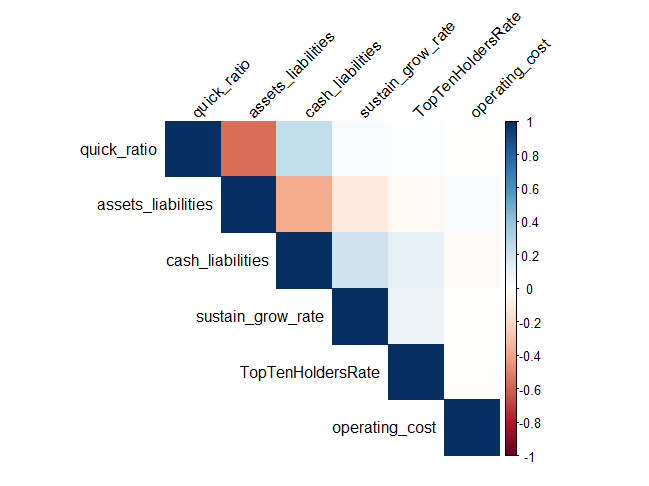
\includegraphics[scale=1]{corrplot}
  \caption{相关系数图} \label{corrplot}
  \end{figure}


% \chapter{附录B}{Appendix B}



% \chapter{附录 C}{Appendix C}
% \begin{figure}[htbp!]
% \centering
% \caption{厦大校徽}
% \xmulogo[0.75]
% \end{figure}
% \begin{figure}[htbp!]
% \centering
% \caption{厦门大学}
% \xmulogon[0.75]
% \end{figure}








\end{document}